\begin{apendices}
  \chapter{\apendseq Notas sobre implementação computacional}\label{apd:notas-sobre-implementacao}

  \section{Estrutura da árvore}\label{sec:estrutura-da-arvore}

Na implementação dos algoritmos descritos nas seções anteriores as árvores são construídas como
estruturas de árvores binárias. Suponha que cada segmento $s_i$ de uma árvore tenha uma 
estrutura conforme ilustrada na Figura~\ref{fig:estrutura-do-segmento}.
Os campos \textit{Up}, \textit{Left} e \textit{Right} vão 
armazenar o índice (isto é, o campo \textit{Index}) dos outros segmentos aos quais $s_i$ estiver conectado 
na árvore. Por convenção, os índices serão números inteiros positivos ou nulo, sendo que quando esses campos 
tiverem o valor $-1$ isso representará que não há conexão. 
Note que $s_i$ poderia 
ser implementado sem o campo \textit{Up}, 
mas esse campo é bastante útil para percorrer o caminho de $s_i$ até o segmento 
raiz da árvore (algo que será necessário várias vezes durante a construção da mesma).
Os campos \textit{Distal point} ($P_i$), \textit{Flow} ($Q_i$), 
\textit{Left bifurcation ratio} ($\beta_i^l$) e \textit{Right bifurcation ratio} ($\beta_i^r$)
são dados do segmento $s_i$ que serão necessários durante os cálculos da 
resistência hidrodinâmica da árvore e do valor da função custo.

\begin{figure}[!htb]
  \centering
  \captiondelim{: }
  \caption{Estrutura de um segmento terminal $s_i$ da árvore binária.}  
  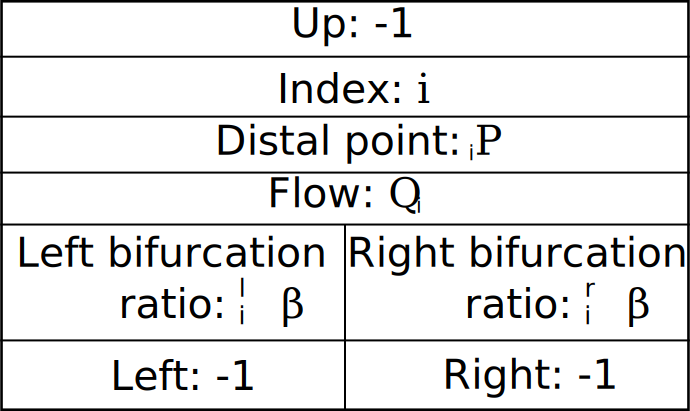
\includegraphics[scale=0.35]{figuras/notas-sobre-implementacao/estrutura-do-segmento.pdf}
  \fonteAutor{2022}
  \label{fig:estrutura-do-segmento}
\end{figure}

Note que os segmentos da árvore binária precisarão ser acessados muitas vezes durante
a execução dos algoritmos. É conveniente que esse acesso possa ser feito de
forma direta através do índice do segmento, evitando assim a necessidade de percorrer a árvore
desde a raiz até chegar no segmento desejado. Além disso, o número total de segmentos da 
árvore já será conhecido desde o início do algoritmo, pois como entrada temos que a árvore 
binária terá $N_{term}$ segmentos terminais. Isso implica que a árvore terá o total de $2N_{term} - 1$
segmentos. Nesse contexto, pode-se alocar na memória os segmentos da árvore binária  
como sendo um vetor $\texttt{segments}$ com $2N_{term} - 1$ posições. Cada posição $\texttt{segments[i]}$ será um ponteiro 
para o segmento $s_i$. A alocação de todos os $2N_{term} - 1$ segmentos pode ser feita logo no início
dos algoritmos, para evitar frequentes alocações/desalocações de memória durante a execução.

Na construção de uma floresta com $N_{trees}$ árvores a quantidade total de segmentos terminais $N_{term}$ 
da floresta é conhecida. Entretanto, não se sabe a priori quantos segmentos terminais cada árvore da floresta 
terá ao final da construção. Para evitar alocação/desalocação de memória durante a construção da floresta, 
pode-se alocar previamente $2N_{term} - 1$ segmentos para cada árvore. Por um lado isso significa 
que haverá espaço alocado que não será utilizado, mas por outro isso simplifica a implementação do algoritmo. 
Aloca-se na memória as árvores como sendo um vetor $\texttt{trees}$ com $N_{trees}$ posições.
Cada posição $\texttt{trees[i]}$ será um ponteiro para a árvore $i$.

Durante a execução do algoritmo será necessário por diversas vezes conhecer o comprimento e o raio 
de um dado segmento $s_i$. O raio pode ser calculado usando as equações~\eqref{eq:raio.segmento.j} e~\eqref{eq:raio.iroot}.
Já o comprimento pode ser calculado através da distância euclidiana entre
o ponto distal $P_i$ de $s_i$ e o ponto distal $P_{parent}$ de $s_{parent}$ que é pai de 
$s_i$ (isto é, quando o campo \textit{Up} de $s_i$ é igual ao campo \textit{Index} de $s_{parent}$). 
A única exceção é o segmento raiz $s_0$, para o qual precisamos calcular a distância euclidiana entre 
seu ponto distal $P_0$ e o ponto $\mathrm{x}_{root}$ (que é a ``semente'' da raiz da árvore fornecida
na entrada do algoritmo). 
Para evitar efetuar esse cálculo várias vezes, podemos armazenar em um vetor $\texttt{length}$ 
esses comprimentos, de tal modo que o comprimento de $s_i$ estará na posição $\texttt{length[i]}$.
Vale notar que $\texttt{length[i]}$ precisa ser atualizado apenas quando $P_i$ ou $P_{parent}$ forem 
alterados.

Por outro lado, todas as vezes que um dado $s_i$ tem seu comprimento alterado isso fará com que seja alterada também 
a resistência hidrodinâmica reduzida $R^*_{sub,\,i}$ da árvore, sendo que seu cálculo é dado pelo equação~\eqref{eq:resistencia.reduzida}.
Novamente para evitar efetuar esse cálculo várias vezes, podemos armazenar em um vetor $\texttt{reducedHydrodynamicResistance}$ 
essas resistências, de tal modo que $R^*_{sub,\,i}$ estará na posição $\texttt{reducedHydrodynamicResistance[i]}$.

  \section{Inicialização da árvore}\label{sec:inicializacao-da-arvore}

O segmento raiz $s_0$ será inserido na inicialização do algoritmo. Esse segmento 
recebe como ponto distal $P_0$ um ponto $\mathrm{x}_{inew}$ dentro do domínio de perfusão.
Os seus campos \textit{Up}, \textit{Left} e \textit{Right} recebem o valor $-1$ e os campos 
$\beta_0^l$ e $\beta_0^r$ recebem o valor $1$. Já o campo 
$Q_0$ recebe $Q_{perf}$ (que é o fluxo de perfusão na entrada da árvore que foi fornecido
como entrada do algoritmo).

O $s_0$ ocupará a posição $\texttt{segments[0]}$, 
sendo que nesse momento inicial o segmento raiz será também o único segmento da árvore.
Calcula-se $\texttt{length[0]}$ como a distância euclidiana entre $P_0$ e o ponto 
$\mathrm{x}_{root}$. Em seguida, calcula-se $\texttt{reducedHydrodynamicResistance[0]}$ usando a equação~\eqref{eq:resistencia.reduzida}. Nesse caso, como há apenas um segmento na árvore, tem-se que 
$\texttt{reducedHydrodynamicResistance[0]}$ receberá o valor $\dfrac{8\eta l_{0}}{\pi}$.

  \section{Segmento da árvore mais próximo de um ponto}\label{sec:vizinhanca-de-um-ponto}

Durante o processo de otimização estrutural (conforme descrito na Seção~\ref{sec:otimizacao-estrutural}) é
necessário localizar até $N_{con}$ segmentos na árvore que estão mais próximos do ponto $\mathrm{x}_{inew}$. 
Para realizar essa tarefa calcula-se a distância crítica~\eqref{eq:dist-critica} entre $\mathrm{x}_{inew}$ 
e cada segmento $s_i$ da árvore. Suponha que essas distâncias sejam armazenadas no vetor 
$\texttt{distance}$. Esse vetor deve ser colocado em ordem decrescente 
utilizando um algoritmo de ordenação, como por exemplo o método da bolha (\textit{bubble sort}). 
Por fim, determina-se os $N_{con}$ segmentos associados à $\texttt{distance[0]}$, $\texttt{distance[1]}$, 
\ldots, $\texttt{distance[}N_{con}\texttt{]}$.

  \section{Inserir segmento terminal na árvore}\label{sec:inserir-segmento-terminal}

Para inserir um novo segmento terminal $s_{i}$ será necessário inserir também um segmento 
de conexão $s_{i-1}$. Por convenção, pode-se inserir cada novo segmento terminal $s_i$ 
sempre na última posição da sequência $\texttt{segments[0]}$, $\texttt{segments[1]}$, \ldots, $\texttt{segments[i-1]}$, $\texttt{segments[i]}$.

A Figura~\ref{fig:exemplo-inserir-segmento} ilustra 
um segmento terminal $s_{i}$ sendo inserido na árvore através
de uma conexão com o segmento $s_c$.
Note que, por convenção, podemos escolher sempre salvar os índices de $s_{i-1}$ e $s_{i}$,
respectivamente, nos campos \textit{Left} e \textit{Right} de $s_c$ (mesmo que geometricamente 
os pontos distais $P_{i-1}$ e $P_{i}$ não estejam, respectivamente, à esquerda e à direita 
do segmento $s_c$).
Além disso, observe que $s_{i-1}$ vai herdar os valores dos campos \textit{Left} e \textit{Right}
que existiam antes em $s_c$. O fluxo $Q_{i-1}$ em $s_{i-1}$ será o mesmo que havia antes em $s_c$ (isto é, 
$Q_{c}$). Já o fluxo $Q_i$ em $s_{i}$ será calculado para um novo segmento terminal.
O fluxo $Q_{c}$ será atualizado como $Q_{i-1} + Q_{i}$.

\begin{figure}[!htb]
  \centering
  \captiondelim{: }
  \caption{Exemplo para inserir um novo segmento terminal $s_{i}$ conectado ao segmento $s_c$.
  (a) Organização da árvore antes de inserir $s_{i}$.
  (b) Organização da árvore depois de inserir $s_{i}$.}
  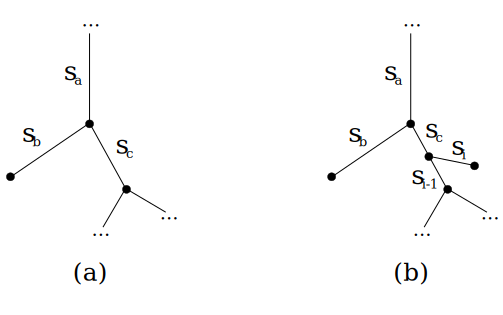
\includegraphics[scale=0.75]{figuras/notas-sobre-implementacao/exemplo-inserir-novo-terminal.pdf}
  \fonteAutor{2022}
  \label{fig:exemplo-inserir-segmento}
\end{figure}

É importante notar que ao inserir $s_{i}$ na árvore o fluxo passando por todo o caminho de 
$s_c$ até a raiz $s_0$ será alterado. Isso significa que os raios de 
todos os segmentos nesse caminho precisam ser atualizados. Ou seja, serão 
recalculadas as razões de bifurcação de todos esses segmentos (conforme descrito na Seção~\ref{sec:ajuste-dos-raios}).
Além disso, como $s_c$ teve seu comprimento alterado e $s_i$ foi inserido na árvore, o valor de 
$R^*_{sub,c}$ deve ser recalculado (o que significa atualizar o valor de $\texttt{reducedHydrodynamicResistance[c]}$).

  \section{Remover segmento terminal na árvore}\label{sec:remover-segmento-terminal}

Para remover um segmento terminal $s_i$ da árvore pode-se atualizar 
os valores dos campos \textit{Left} e \textit{Right} do seu segmento pai $s_c$
de modo a coincidirem com os mesmos valores desses campos do segmento de conexão $s_{i-1}$. 
Além disso, o ponto distal de $s_c$ passará a ser o ponto distal de $s_{i-1}$. 
O fluxo $Q_{c}$ em $s_{c}$ será o mesmo que havia em $s_{i-1}$ (isto é, $Q_{i-1}$). 
Por fim, será necessário recalcular 
as razões de bifurcação de todos os segmentos no caminho de $s_c$ até a raiz $s_0$, 
bem como atualizar o valor de $\texttt{reducedHydrodynamicResistance[c]}$.

\end{apendices}